% Template for ICASSP-2020 paper; to be used with:
%          spconf.sty  - ICASSP/ICIP LaTeX style file, and
%          IEEEbib.bst - IEEE bibliography style file.
% --------------------------------------------------------------------------
\documentclass{article}
\usepackage{spconf,amsmath,graphicx}

% Example definitions.
% --------------------
\def\x{{\mathbf x}}
\def\L{{\cal L}}

% Title.
% ------
\title{IMPLEMENTING AN OBJECTIVE FUNCTION AND REPORTING THE EFFECTS OF REGULARISATION ON GENERATIVE MODELS}
%
% Single address.
% ---------------
\name{Chad Kakau \thanks{AIML425}}
\address{Victoria University, Wellington}
%
%
\begin{document}
%\ninept
%
\maketitle
%
\begin{abstract}
this paper revises the concept of objective functions as applied in machine learning and identifies the SELECTED OBJECTIVE FUNCTION used by the authors in the implementation of a generative neural network.  The generative model maps a gaussian distribution to a uniform distribution, then maps the uniform distribution to a gaussian distribution, for a concatenated gaussian to gaussian network.  This paper lists the three main objective functions used in neural networks and \bf{SOMETHING TO SAY GOES THROUGH THE MATH of the selected function:  .}  The results of the implemented neural network show that 
\end{abstract}
%
\begin{keywords}
One, two, three, four, five
\end{keywords}
%
\section{Introduction}
\label{sec:intro}
%
These guidelines include complete descriptions of the fonts, spacing, and
related information for producing your proceedings manuscripts. Please follow
them and if you have any questions, direct them to Conference Management
Services, Inc.: Phone +1-979-846-6800 or email
to \\\texttt{icassp2020@cmsworkshops.com}.

\section{Objective functions and regularisation}
\label{sec:format}

The theory:  
Why obective functions?
- machine learning applies models to iteratively improve performance at generating a desired output (ref)
- improves by 'moving' actual outputs closer to desired outputs, using an objective function tht calculates the difference or similarity between the actual output an the desired output
- can be applied at the level of individual instances or across the distribution of input and output sets
why regularisation?
- list the options and distinguish between the options (method, output, application)
- link the selected option with this problem 
  - which will be the best for low/high outliers
  - which will be the best for 
which objective function?

- map the math
- 

%
\section{RESULTS}
\label{sec:results}
%


\subsection{Subheadings}
\label{ssec:subhead}

\subsubsection{Sub-subheadings}
\label{sssec:subsubhead}


\section{ILLUSTRATIONS, GRAPHS, AND PHOTOGRAPHS}
\label{sec:illust}

Since there are many ways, often incompatible, of including images (e.g., with
experimental results) in a LaTeX document, below is an example of how to do
this \cite{Lamp86}.

% Below is an example of how to insert images. Delete the ``\vspace'' line,
% uncomment the preceding line ``\centerline...'' and replace ``imageX.ps''
% with a suitable PostScript file name.
% -------------------------------------------------------------------------
\begin{figure}[htb]

\begin{minipage}[b]{1.0\linewidth}
  \centering
  \centerline{
\includegraphics[width=8.5cm]{image1}}
%  \vspace{2.0cm}
  \centerline{(a) Result 1}\medskip
\end{minipage}
%
\begin{minipage}[b]{.48\linewidth}
  \centering
  \centerline{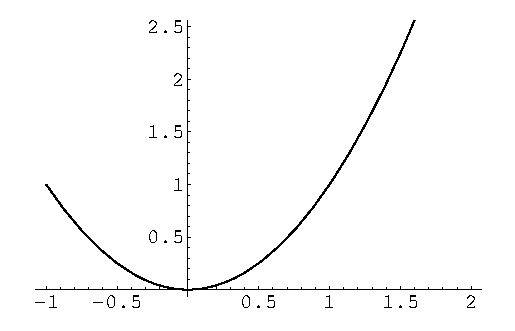
\includegraphics[width=4.0cm]{image3}}
%  \vspace{1.5cm}
  \centerline{(b) Results 3}\medskip
\end{minipage}
\hfill
\begin{minipage}[b]{0.48\linewidth}
  \centering
  \centerline{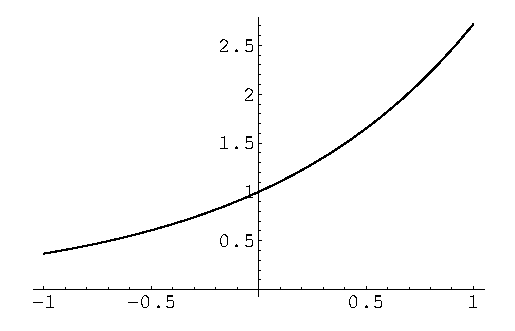
\includegraphics[width=4.0cm]{image4}}
%  \vspace{1.5cm}
  \centerline{(c) Result 4}\medskip
\end{minipage}
%
\caption{Example of placing a figure with experimental results.}
\label{fig:res}
%
\end{figure}


% To start a new column (but not a new page) and help balance the last-page
% column length use \vfill\pagebreak.
% -------------------------------------------------------------------------
%\vfill
%\pagebreak

\section{CONCLUSION}
\label{sec:CONC}

Here is a citation \cite{C2}. 

% References should be produced using the bibtex program from suitable
% BiBTeX files (here: strings, refs, manuals). The IEEEbib.bst bibliography
% style file from IEEE produces unsorted bibliography list.
% -------------------------------------------------------------------------

%\vfill\pagebreak

\bibliographystyle{IEEEbib}
\bibliography{strings,refs}

\end{document}
